\documentclass{beamer}

\usepackage{listings}
\usepackage[utf8]{inputenc}
\usetheme{Madrid}
\setbeamersize{text margin left=0.1\textwidth,text margin right=0.1\textwidth}
\setbeamertemplate{section in toc}{\inserttocsection}
\lstset{language=python,
        keywordstyle=\color{red},
        basicstyle=\ttfamily,
        basicstyle=\small,
        frame = single,
        framexleftmargin=15pt,
        numbers=left, 
        numberstyle=\small, 
        numbersep=5pt, 
        xleftmargin=0.05\textwidth,
        columns=fullflexible}

%Information to be included in the title page:
\title{Advanced MapReduce}
\author{Cary Goltermann}
\institute{Galvanize}
\date{2016}

\AtBeginSubsection[]
{
  \begin{frame}
    \frametitle{Overview}
    \tableofcontents[currentsection,currentsubsection]
  \end{frame}
}
 
\begin{document}
 
\frame{\titlepage}

\begin{frame}
  \frametitle{Overview}
  \tableofcontents[]
\end{frame}

\section{Advanced MapReduce}
\begin{frame}
  \frametitle{MapReduce}
  \parbox{\linewidth}{MapReduce deals with most of the details of distributed computing (the ones that we would otherwise like to not think about) and automatically handles most of the concerns with:}
  \vspace{4mm}
  \begin{itemize}
    \item Parallelization and distribution of data and computation
    \item Fault-tolerance
    \item Resource management
    \item Status monitoring
  \end{itemize}
\end{frame}

\subsection{Shuffle and Sort}
\begin{frame}
  \frametitle{Shuffle and Sort}
  \parbox{\linewidth}{How data is re-distributed during a MapReduce job to continually take advantage of all the worker nodes.} \vspace{2mm}
  \begin{columns}
    \column{0.5\textwidth}
    \begin{center}
      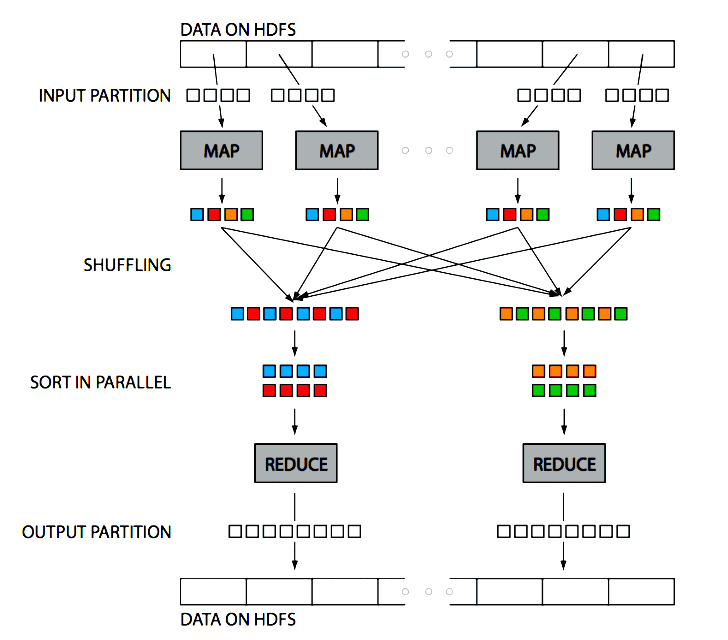
\includegraphics[width=\textwidth]{../images/shuffle_sort.png}
    \end{center}
    \column{0.5\textwidth}
    \begin{itemize}
      \item \alert{Shuffle Step}: Process of deciding how and where data from mappers will go to the reducers.
      \vspace{1mm}
      \item \alert{Sort Step}: Sorts data it gets from the mappers by key.
    \end{itemize}
  \end{columns}
\end{frame}

\begin{frame}
  \frametitle{Tracking}
  \begin{center}
    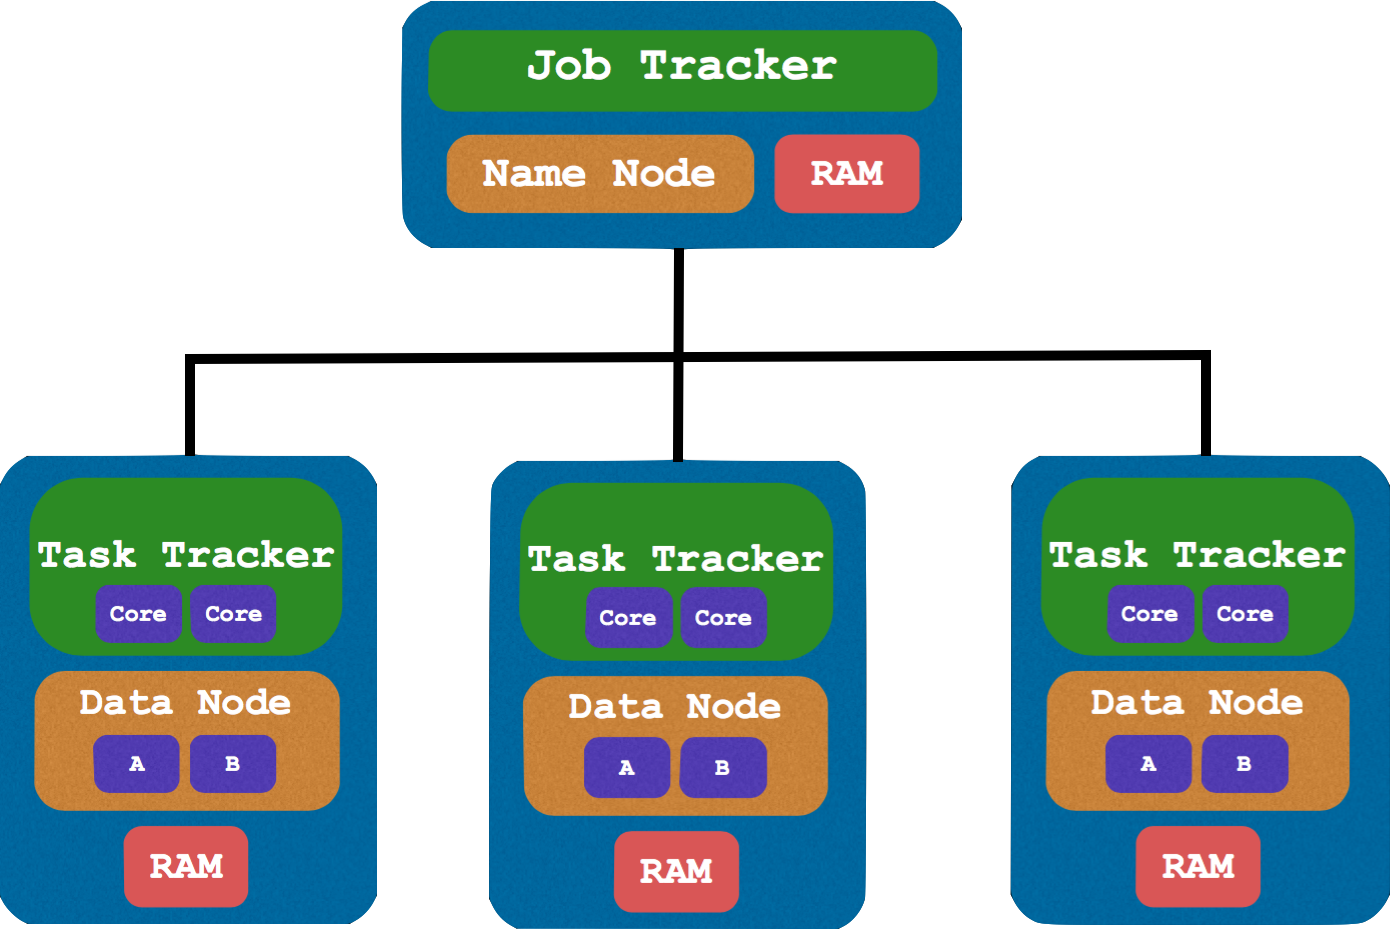
\includegraphics[width=\textwidth]{../images/tracking.png}
  \end{center}
\end{frame}

\begin{frame}
  \frametitle{Partitioning}
  \begin{center}
    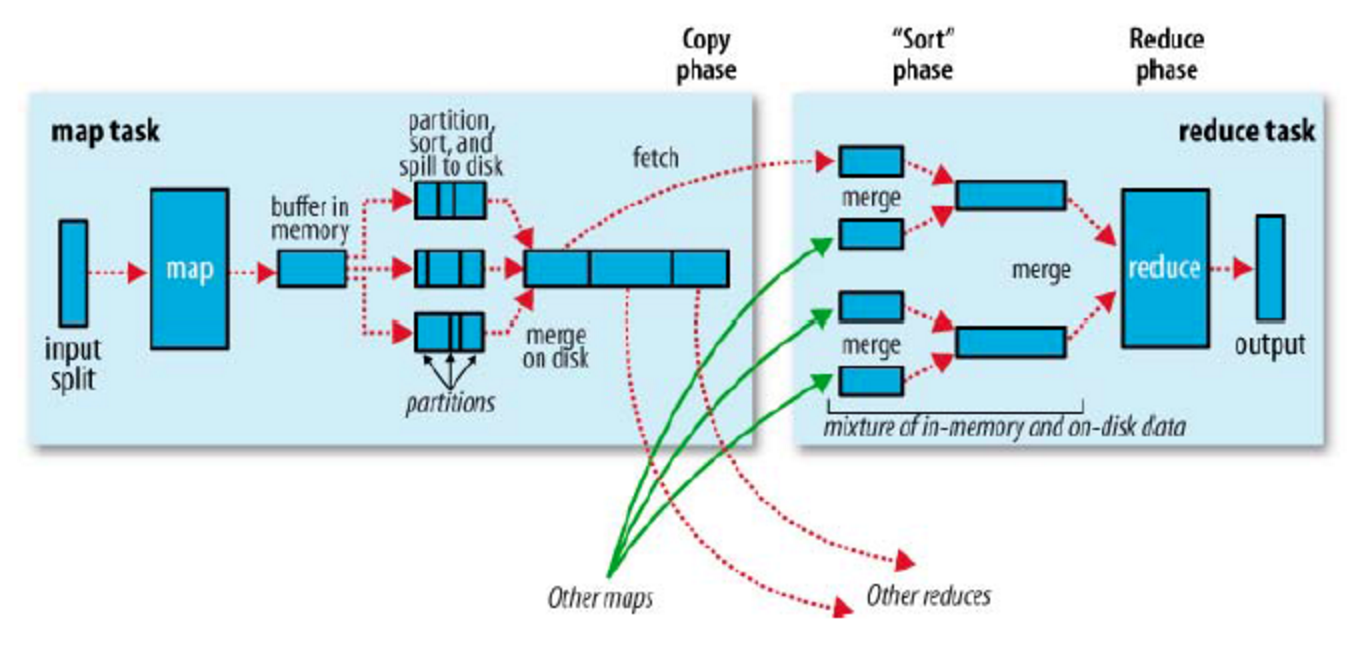
\includegraphics[width=\textwidth]{../images/partitioning.png}
  \end{center}

    \parbox{\linewidth}{\small The partitioner on each mapper takes care of any local sorting it can do to the data it's outputting and the reducers take care of merging all the sorted partitions that get sent to them during the shuffle.}
\end{frame}

\begin{frame}
  \frametitle{Scarce Resources}
    In a distributed computing framework like Hadoop what is one of the most scarce resources? \pause
  \vspace{2mm}
  \begin{alertblock}{Bandwidth}
    The time cost of transmitting data around the cluster, between nodes, as in the shuffle and sort step, is quite high.
  \end{alertblock} \pause
  \vspace{4mm}
  \parbox{\linewidth}{What if we could decrease the amount of data we have to move in our shuffle and sort, or eliminate it all together?}
\end{frame}

\subsection{Counters}
\begin{frame}[fragile]
  \frametitle{Counters}
  \begin{itemize}
    \item Used to keep track of events that occur over a given map or reduce step.
    \item Mostly used for debugging purposes. E.g. To verify that all of the folders in your file system are getting accessed correctly.
  \end{itemize} \vspace{2mm}
  \begin{lstlisting}
  class MRCountingJob(MRJob):

      def mapper(self, _, value):
          self.increment_counter('group', 'counter_name', 1)
              yield _, value
  \end{lstlisting}
\end{frame}

\begin{frame}[fragile]
  \frametitle{Counters Code}
  \parbox{\linewidth}{Counters can also be used to avoid using a reducer in some cases. If all you're trying to do is count by some key then a counter can help you avoid the time consuming process of the shuffle and sort when you use a reducer.}
  \vspace{2mm}
  \begin{lstlisting}
  import os

  class MRWordCount(MRJob):
    
      def mapper(self, _, line):
          filepath = os.environ['map_input_file']
          filename = filepath.split('/')[-1]

          for word in line.split():
              self.increment_counter(filename, 'word_counts', 1)
  \end{lstlisting}
\end{frame}

\subsection{Combiners}
\begin{frame}
  \frametitle{Combiners}
  \begin{itemize}
    \item Help decrease the amount of data that needs to be passed from mappers to reducers.
    \item Frequently look like reducers that aggregate like data on the mapper so that there is "less" of it to copy to the reducers.
    \item \alert{Note}: The same information needs to get passed to the reducers no matter what, combiners generally find a way to achieve this while using fewer bits to represent that information.
  \end{itemize}
\end{frame}

\begin{frame}
  \frametitle{Combiner Example Illustrated}
  Let's take a look at an example that illustrates unnecessarily moving data. \pause
  \begin{center}
    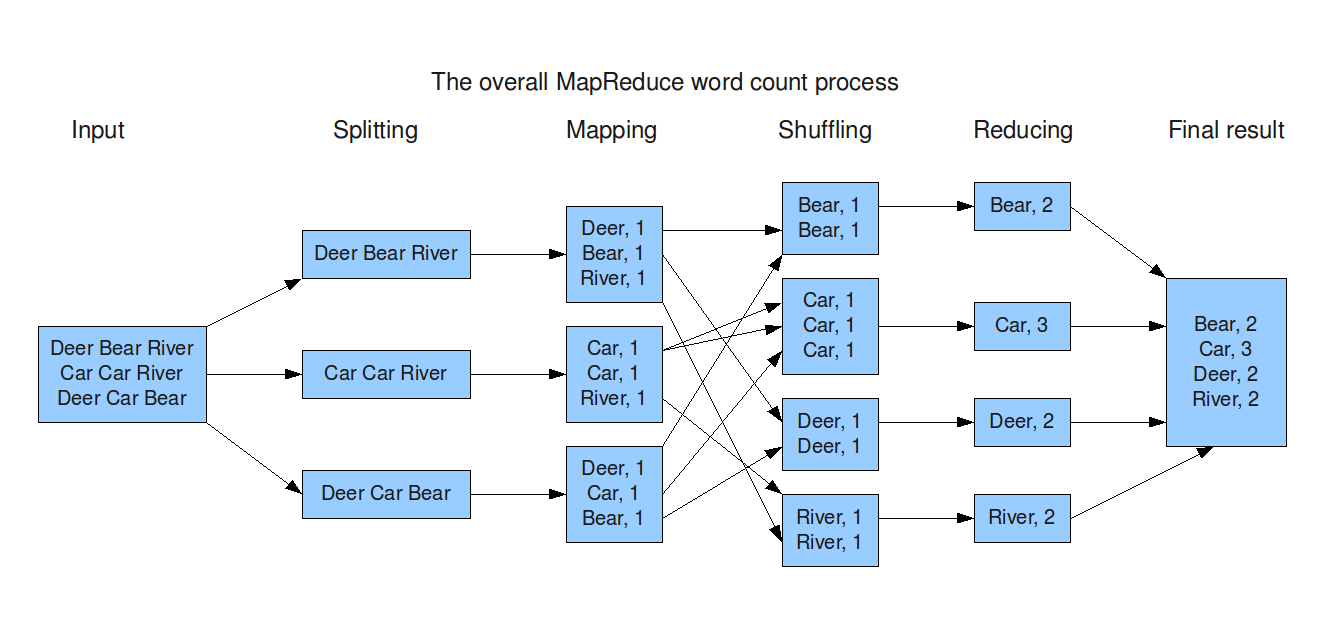
\includegraphics[width=0.8\textwidth]{../images/word_count.png} \pause
  \end{center}
  Does anything strike you as inefficient about this MapReduce implementation?
\end{frame}

\begin{frame}[fragile]
  \frametitle{Combiner Code}
  \begin{lstlisting}
  from string import punctuation

  class MRWordCount(MRJob):
    
      def mapper(self, _, line):
          for word in line.split():
            yield (word.strip(punctuation).lower(), 1)

      def combiner(self, word, counts):
          yield (word, sum(counts))

      def reducer(self, word, counts):
          yield (word, sum(counts))
  \end{lstlisting}
  \alert{Note}: While the combiner and the reducer implement the same function in this example, this is not generally the case when using a combiner.
\end{frame}

\section{Hadoop Ecosystem Tools}
\subsection{Hbase, Hive, Pig}
\begin{frame}
  \frametitle{Hadoop Ecosystem}
  \begin{center}
    
\includegraphics[height=0.25\textheight]{../images/hbase.png}
    \vspace{4mm}
    \begin{columns}
      \column{0.5\textwidth}
      \begin{center}
        
\includegraphics[height=0.3\textheight]{../images/hive.png}
      \end{center}
      \column{0.5\textwidth}
      \begin{center}
        
\includegraphics[height=0.3\textheight]{../images/pig.png}
        \\ {\LARGE Pig}
      \end{center}
    \end{columns}
  \end{center}
\end{frame}

\begin{frame}
  \frametitle{All of the Tools}
  \begin{description}
    \item[Hbase] A mutable big data storage system on top of HDFS. \alert{Note}: HDFS is mutable, batch oriented.
    \item[Hive] A high level language for writing MapReduce jobs in an SQL style.
    \item[Pig] Another high level language for writing MapReduce jobs in. Kind of like Hive, but with less structure and less familiarity from SQL.


  \end{description}
\end{frame}

\end{document}
